\documentclass{article}

%%%%
% PLOTS mapas
% eval=FALSE
% results=HIDE (verbatim default)
%%%%
\usepackage{rotating}
\usepackage[utf8]{inputenc}
\usepackage{longtable}
\usepackage{authblk}
\usepackage{adjustbox}


\title{LOS INDICES DEL MUNDO}
% autores
\renewcommand\Authand{, y }
\author[1]{\normalsize Estrella DelCurso}
\author[2]{\normalsize Prossimo Deal Lado}

\affil[1,2]{\small  Escuela de Ingeniería,Universidad de la vida\\
\texttt{{delcurso,deallado}@vida.edu}}
\affil[1]{\small Instituto de altas investigaciones financieras\\
Banco del Parque\\
\texttt{delcurso@bp.com}}

\date{}

%%%%
\usepackage{Sweave}
\begin{document}
\Sconcordance{concordance:paperVersion_5.tex:paperVersion_5.Rnw:%
1 29 1 1 0 26 1 1 6 3 1 1 12 42 0 1 2 11 1 1 35 1 2 6 1 1 7 12 0 1 2 1 %
7 15 0 1 2 5 1 1 8 13 0 1 2 7 1 1 8 11 0 1 2 6 1 1 4 1 2 11 1 1 5 1 1 1 %
3 37 0 1 2 6 1 1 6 8 0 1 2 2 4 1 5 3 1 1 3 1 2 5 1}


\maketitle


\begin{abstract}
Este es mi primer trabajo en exploracion y modelamiento de indices usando LATEX. Este trabajo lo he hecho bajo la filosofía de trabajo replicable. Este es mi primer trabajo en exploracion y modelamiento de indices usando LATEX. Este trabajo lo he hecho bajo la filosofía de trabajo replicable. Este es mi primer trabajo en exploracion y modelamiento de indices usando LATEX. Este trabajo lo he hecho bajo la filosofía de trabajo replicable. Este es mi primer trabajo en exploracion y modelamiento de indices usando LATEX. Este trabajo lo he hecho bajo la filosofía de trabajo replicable.
\end{abstract}

\section*{Introducción}

Aqui les presento mi investigacion sobre diversos indices sociales en el mundo. Los indices los conseguí de wikipedia, espero que les gusten mucho. Aqui les presento mi investigacion sobre diversos indices sociales en el mundo. Los indices los conseguí de wikipedia, espero que les gusten mucho.Aqui les presento mi investigacion sobre diversos indices sociales en el mundo. Los indices los conseguí de wikipedia, espero que les gusten mucho.Aqui les presento mi investigacion sobre diversos indices sociales en el mundo. Los indices los conseguí de wikipedia, espero que les gusten mucho.
Aqui les presento mi investigacion sobre diversos indices sociales en el mundo. Los indices los conseguí de wikipedia, espero que les gusten mucho.Aqui les presento mi investigacion sobre diversos indices sociales en el mundo. Los indices los conseguí de wikipedia, espero que les gusten mucho.Aqui les presento mi investigacion sobre diversos indices sociales en el mundo. Los indices los conseguí de wikipedia, espero que les gusten mucho.

Comencemos viendo que hay en la sección \ref{univariada} en la página \pageref{univariada}.

\clearpage



\section{Exploración Univariada}\label{univariada}

En esta sección exploro cada índice. En esta sección exploro cada índice. En esta sección exploro cada índice. En esta sección exploro cada índice. En esta sección exploro cada índice. En esta sección exploro cada índice. En esta sección exploro cada índice. En esta sección exploro cada índice. En esta sección exploro cada índice.





Para conocer el comportamiento de las variables se ha preparado la Tabla \ref{Tfrecuencias}, donde se describe la distribución de las modalidades de cada variable. Los números representan la situación de algun país en ese indicador, donde el mayor valor numérico es la mejor situación.

% latex table generated in R 3.5.0 by xtable 1.8-3 package
% Fri Nov 23 21:00:31 2018
\begingroup\normalsize
\begin{longtable}{llrrr}
\caption{Tablas de Frecuencia de la variables en estudio} \\ 
 \textbf{Variable} & \textbf{Levels} & $\mathbf{n}$ & $\mathbf{\%}$ & $\mathbf{\sum \%}$ \\ 
  \hline \hline
WorldFreedom & 1 very bad & 46 & 24.7 & 24.7 \\ 
   & 3 middle & 56 & 30.1 & 54.8 \\ 
   & 5 very good & 84 & 45.2 & 100.0 \\ 
   \hline
 & all & 186 & 100.0 &  \\ 
   \hline
\hline
EconomicFreedom & 1 very bad & 18 & 9.7 & 9.7 \\ 
   & 2 bad & 65 & 35.0 & 44.6 \\ 
   & 3 middle & 71 & 38.2 & 82.8 \\ 
   & 4 good & 26 & 14.0 & 96.8 \\ 
   & 5 very good & 6 & 3.2 & 100.0 \\ 
   \hline
 & all & 186 & 100.0 &  \\ 
   \hline
\hline
PressFreedom & 1 very bad & 20 & 10.8 & 10.8 \\ 
   & 2 bad & 44 & 23.7 & 34.4 \\ 
   & 3 middle & 60 & 32.3 & 66.7 \\ 
   & 4 good & 45 & 24.2 & 90.9 \\ 
   & 5 very good & 17 & 9.1 & 100.0 \\ 
   \hline
 & all & 186 & 100.0 &  \\ 
   \hline
\hline
Democracy & 1 very bad & 50 & 26.9 & 26.9 \\ 
   & 2 bad & 40 & 21.5 & 48.4 \\ 
   & 4 good & 77 & 41.4 & 89.8 \\ 
   & 5 very good & 19 & 10.2 & 100.0 \\ 
   \hline
 & all & 186 & 100.0 &  \\ 
   \hline
\hline
\hline
\label{Tfrecuencias}
\end{longtable}
\endgroup

Como apreciamos en la Tabla \ref{Tfrecuencias}, los países en la mejor situación son los menos, salvo en el caso del \emph{índice de libertas mundial}\footnote{Nótese que esto se puede deber a la {\bf menor} cantidad de categorías.}

\clearpage

Para resaltar lo anterior, tenemos la Figura \ref{barplots} en la página \pageref{barplots}. 


%%%%% figure
\begin{figure}[h]
\centering
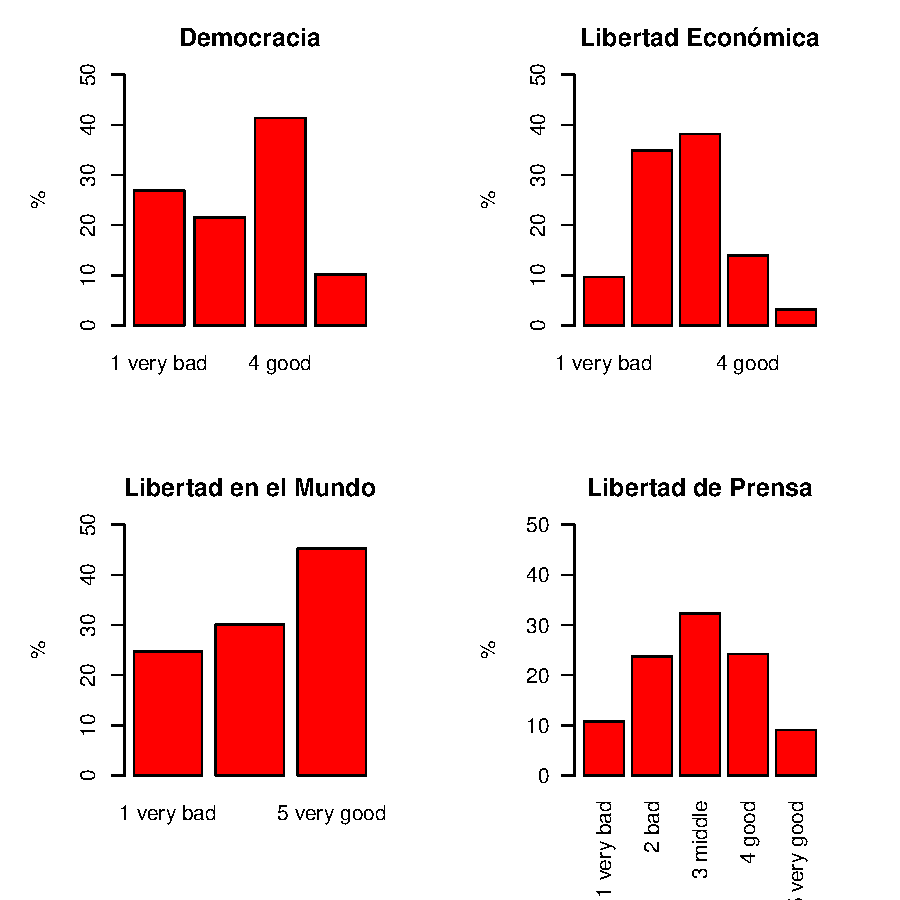
\includegraphics{paperVersion_5-barplots}
\caption{Distribución de Indicadores}
\label{barplots}
\end{figure}

Además de la distribución de los variable, es importante saber el valor central y otros estadísticos. La Tabla \ref{statsnum} de la página \pageref{statsnum} y la Tabla \ref{statsord} de la página \pageref{statsord} nos muestran los estadísticos apropiados segun el tipo de variable.


% Table created by stargazer v.5.2.2 by Marek Hlavac, Harvard University. E-mail: hlavac at fas.harvard.edu
% Date and time: Fri, Nov 23, 2018 - 21:00:31
\begin{table}[!htbp] \centering 
  \caption{Estadísticos para variables numéricas} 
  \label{statsnum} 
\begin{tabular}{@{\extracolsep{5pt}}lccccc} 
\\[-1.8ex]\hline 
\hline \\[-1.8ex] 
Statistic & \multicolumn{1}{c}{N} & \multicolumn{1}{c}{Mean} & \multicolumn{1}{c}{Median} & \multicolumn{1}{c}{Min} & \multicolumn{1}{c}{Max} \\ 
\hline \\[-1.8ex] 
gdp & 186 & 21,667.200 & 13,000 & 700 & 139,100 \\ 
\hline \\[-1.8ex] 
\end{tabular} 
\end{table} 
% Table created by stargazer v.5.2.2 by Marek Hlavac, Harvard University. E-mail: hlavac at fas.harvard.edu
% Date and time: Fri, Nov 23, 2018 - 21:00:31
\begin{table}[!htbp] \centering 
  \caption{Estadísticos para variables ordinales} 
  \label{statsord} 
\begin{tabular}{@{\extracolsep{5pt}}lcccc} 
\\[-1.8ex]\hline 
\hline \\[-1.8ex] 
Statistic & \multicolumn{1}{c}{N} & \multicolumn{1}{c}{Median} & \multicolumn{1}{c}{Max} & \multicolumn{1}{c}{Min} \\ 
\hline \\[-1.8ex] 
FreedomintheWorld & 186 & 3 & 5 & 1 \\ 
IndexofEconomicFreedom & 186 & 3 & 5 & 1 \\ 
PressFreedomIndex & 186 & 3 & 5 & 1 \\ 
DemocracyIndex & 186 & 4 & 5 & 1 \\ 
\hline \\[-1.8ex] 
\end{tabular} 
\end{table} 

\section{Exploración Bivariada}

En este trabajo estamos interesados en el impacto de los otros indices en el nivel de Democracia. Veamos las relaciones bivariadas que tiene esta variable con todas las demás:

% Table created by stargazer v.5.2.2 by Marek Hlavac, Harvard University. E-mail: hlavac at fas.harvard.edu
% Date and time: Fri, Nov 23, 2018 - 21:00:31
\begin{table}[!htbp] \centering 
  \caption{Correlación de GDP con las demás variables} 
  \label{corrDem} 
\begin{tabular}{@{\extracolsep{5pt}} cc} 
\\[-1.8ex]\hline 
\hline \\[-1.8ex] 
FreedomintheWorld & $0.247$ \\ 
IndexofEconomicFreedom & $0.588$ \\ 
PressFreedomIndex & $0.328$ \\ 
DemocracyIndex & $0.356$ \\ 
\hline \\[-1.8ex] 
\end{tabular} 
\end{table} 

Veamos la correlación entre las variables independientes:


\begin{sidewaystable}
\centering
\caption{Correlación entre variables independientes}
% Table created by stargazer v.5.2.2 by Marek Hlavac, Harvard University. E-mail: hlavac at fas.harvard.edu
% Date and time: Fri, Nov 23, 2018 - 21:00:31
\begin{tabular}{@{\extracolsep{5pt}} ccccc} 
\\[-1.8ex]\hline 
\hline \\[-1.8ex] 
 & FreedomintheWorld & IndexofEconomicFreedom & PressFreedomIndex & DemocracyIndex \\ 
\hline \\[-1.8ex] 
FreedomintheWorld & 1 &  &  &  \\ 
IndexofEconomicFreedom & 0.48 & 1 &  &  \\ 
PressFreedomIndex & 0.83 & 0.52 & 1 &  \\ 
DemocracyIndex & 0.89 & 0.58 & 0.76 & 1 \\ 
\hline \\[-1.8ex] 
\end{tabular} \end{sidewaystable}

Lo visto en la Tabla \ref{corrTableX} se refuerza claramente en la Figura \ref{corrPlotX}.

\begin{figure}[h]
\centering
\begin{adjustbox}{width=7cm,height=7cm,clip,trim=1.5cm 0.5cm 0cm 1.5cm}
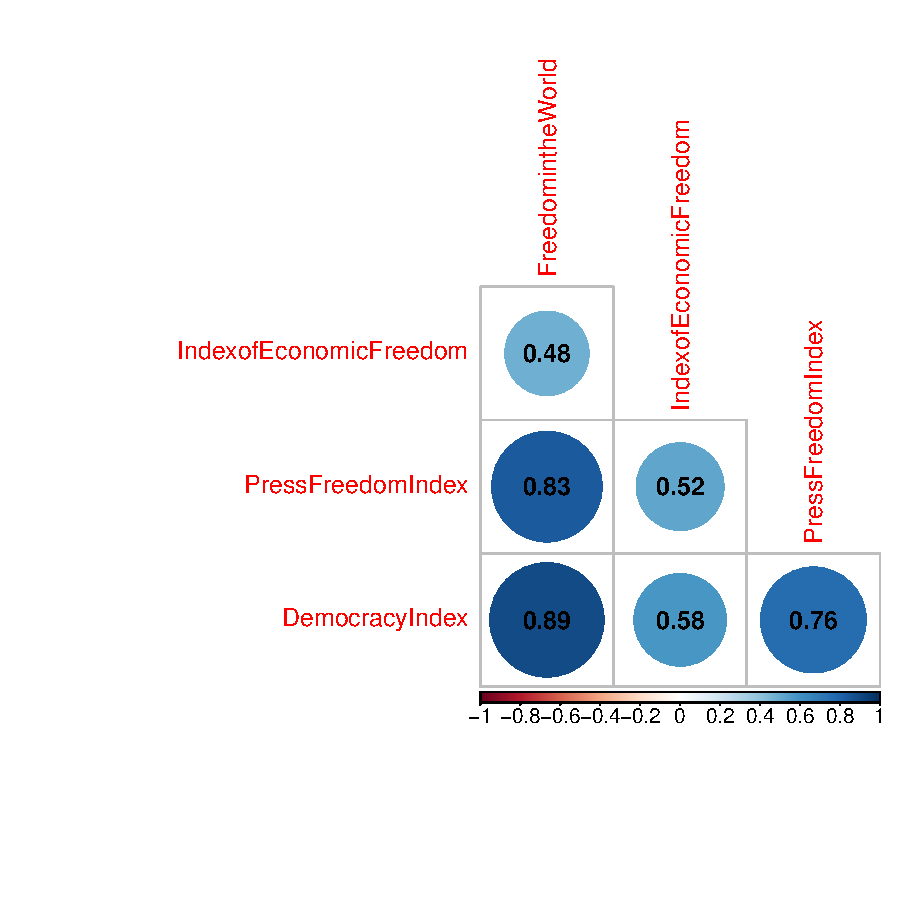
\includegraphics{paperVersion_5-corrPlotX}
\end{adjustbox}
\caption{correlación entre predictores}
\label{corrPlotX}
\end{figure}


\clearpage

\section{Modelos de Regresión}

FFinalmente, vemos los modelos propuestos. Primero sin el índice de democracia como independiente, y luego con éste. Los resultados se muestran en la Tabla \ref{regresiones} de la página \pageref{regresiones}.



% Table created by stargazer v.5.2.2 by Marek Hlavac, Harvard University. E-mail: hlavac at fas.harvard.edu
% Date and time: Fri, Nov 23, 2018 - 21:00:31
\begin{table}[!htbp] \centering 
  \caption{Modelos de Regresión} 
  \label{regresiones} 
\begin{tabular}{@{\extracolsep{5pt}}lcc} 
\\[-1.8ex]\hline 
\hline \\[-1.8ex] 
 & \multicolumn{2}{c}{\textit{Dependent variable:}} \\ 
\cline{2-3} 
\\[-1.8ex] & \multicolumn{2}{c}{gdp} \\ 
\\[-1.8ex] & (1) & (2)\\ 
\hline \\[-1.8ex] 
 FreedomintheWorld & $-$2,582.285 & $-$5,505.874$^{**}$ \\ 
  & (1,579.153) & (2,305.879) \\ 
  & & \\ 
 IndexofEconomicFreedom & 14,823.900$^{***}$ & 13,575.000$^{***}$ \\ 
  & (1,779.269) & (1,910.907) \\ 
  & & \\ 
 PressFreedomIndex & 3,569.733 & 3,570.992 \\ 
  & (2,326.908) & (2,314.236) \\ 
  & & \\ 
 DemocracyIndex &  & 4,103.246$^{*}$ \\ 
  &  & (2,369.556) \\ 
  & & \\ 
 Constant & $-$19,594.750$^{***}$ & $-$18,067.700$^{***}$ \\ 
  & (4,707.167) & (4,763.864) \\ 
  & & \\ 
\hline \\[-1.8ex] 
Observations & 186 & 186 \\ 
R$^{2}$ & 0.355 & 0.366 \\ 
Adjusted R$^{2}$ & 0.345 & 0.352 \\ 
Residual Std. Error & 19,424.840 (df = 182) & 19,319.060 (df = 181) \\ 
F Statistic & 33.455$^{***}$ (df = 3; 182) & 26.117$^{***}$ (df = 4; 181) \\ 
\hline 
\hline \\[-1.8ex] 
\textit{Note:}  & \multicolumn{2}{r}{$^{*}$p$<$0.1; $^{**}$p$<$0.05; $^{***}$p$<$0.01} \\ 
\end{tabular} 
\end{table} 
\clearpage

\section{Exploración Espacial}

Estos son los lugares donde tenemos información:

\begin{Schunk}
\begin{Soutput}
OGR data source with driver: ESRI Shapefile 
Source: "/cloud/project/world_map/world_map.shp", layer: "world_map"
with 246 features
It has 11 fields
Integer64 fields read as strings:  POP2005 
\end{Soutput}
\end{Schunk}




\begin{figure}[h]
\centering
\begin{adjustbox}{width=11cm,height=8cm,clip,trim=1.5cm 2.5cm 0cm 2.5cm}
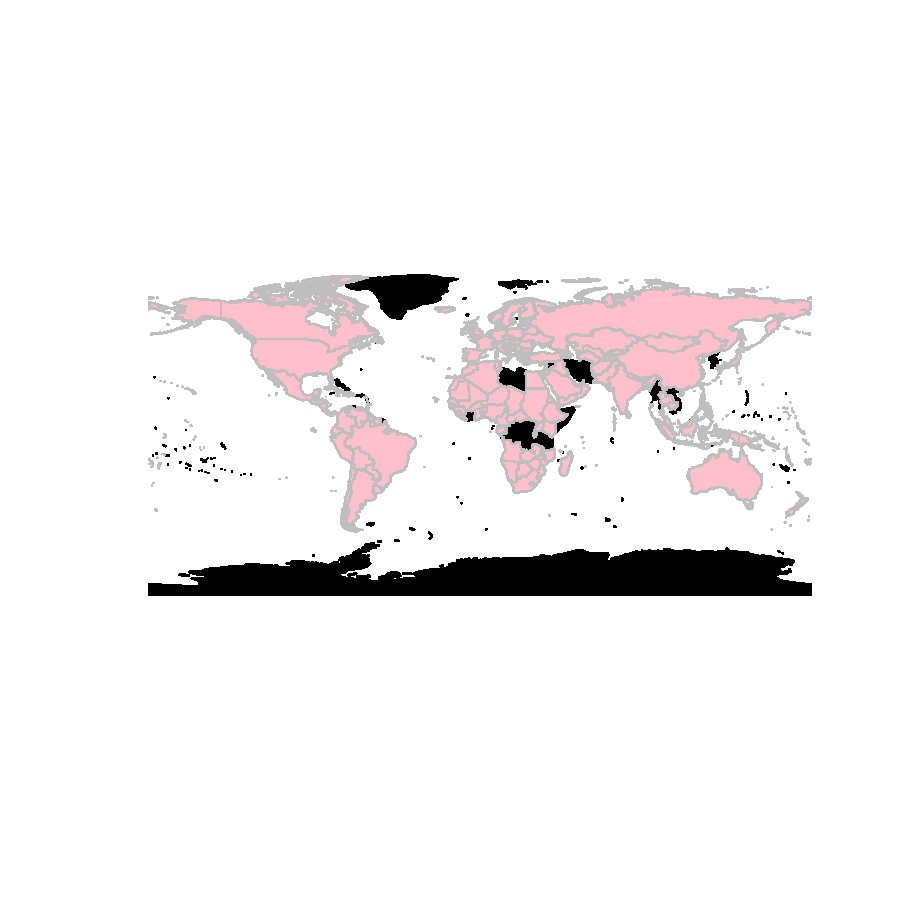
\includegraphics{paperVersion_5-plotMap1}
\end{adjustbox}
\caption{Paises con información diponible}\label{rawmap}
\end{figure}


\end{document}
